% !TEX root =  ../main.tex 

\section{Simulation study}
\label{sec: simulation_study}
For contrasting the personalized scheduling approaches against the schedule of PRIAS and the schedule of doing biopsy every year, we performed a simulation study. We used the parameters from the joint model fitted to the original PRIAS data set to generate 60 data sets with 1000 patients each. We employed a Weibull baseline hazard while generating Gleason reclassification times for the simulated patients. We divided the 60 data sets into groups of 10 each, and within each group the parameter values for the Weibull baseline hazard were kept the same, while across the group they were different. The reason to create such groups was to ensure the consistency of results within in each group. Using different parameter values for the baseline hazard across the groups ensured that we tested not only the scenarios in which patients have early progression times but also those in which patients have late progression times. This is important because how late/early patients are observed to have Gleason reclassification, partially depends on the induction criteria of the AS program.

\subsection{Simulation setup}
\label{subsec : simulation_setup}
We divided each of the 60 data sets into training (750 patients) and test (250 patients) parts. We fitted a joint model to the training data set and using it we generated biopsy schedules for patients in the test data set. Since we generate the true Gleason reclassification time for each of the patients in the test data set, we are able to calculate the offset for each patient and each scheduling method. While creating the personalized schedules we adhere to the PSA measurement schedule of PRIAS. On every visit for the PSA we calculate the time of conducting a biopsy using the scheduling methods given in section \ref{sec : personalized_scheduling}. We call it the proposed time of biopsy. We observed in section \ref{sec : pers_schedule_PRIAS} that in many cases the proposed time of biopsy was postponed on each visit for PSA. In some cases two biopsies within a 1 year period were also proposed, which is not practical. Lastly, since the existence of PSA does not depend on Gleason reclassification, in some cases the proposed time was also earlier than the visit time. To avoid these problems altogether we use the following algorithm to select the time of biopsies from the proposed times.\\

\begin{tikzpicture}
\node (start) [startstop] {Enter Active Surveillance.\\ Perform a biopsy\\Set EnforcedBiopsyTime = $\infty$.\\Set LastBiopsyTime=0.};

\node (propTime) [process, below=1cm of start] {PSA measurement visit.\\Compute ProposedBiopsyTime using a personalized scheduling method.};

\node (decision1) [decision, below = 1cm of propTime] {Is ProposedBiopsyTime earlier than EnforcedBiopsyTime?};

\node (decision5) [decision, left=1cm of decision1] {Is ProposedBiopsyTime is earlier than the current PSA measurement visit time?};

\node (pro5) [process, below=1cm of decision5] {Set ProposedBiopsyTime = CurrentVisitTime};

\node (decision2) [decision, below=1cm of pro5] {Is ProposedBiopsyTime is at least 1 year later than LastBiopsyTime?};

\node (pro2) [process, below=1cm of decision1] {Set EnforcedBiopsyTime = ProposedBiopsyTime};

\node (decision4) [decision, right=1cm of decision1] {Is EnforcedBiopsyTime earlier than next PSA visit time?};

\node (pro3) [process, right=1cm of decision2] {Perform Biopsy at LastBiopsyTime + 1 year};

\node (pro4) [process, below=1cm of decision4] {Perform Biopsy at EnforcedBiopsyTime};

\node (decision3) [decision, below=1cm of pro3] {Is Gleason score greater than 6?};

\node (stop) [startstop, below = 1cm of decision3] {Remove patient from AS};


\draw [arrow] (start) -- (propTime);
\draw [arrow] (propTime) -- (decision1);
\draw [arrow] (decision1) -- node[anchor=south] {Yes} (decision5);
\draw [arrow] (decision5) -- node[anchor=east] {Yes} (pro5);
\draw [arrow] (pro5) -- (decision2);
\draw [arrow] (decision1) -- node[anchor=south] {No} (decision4);
\draw [arrow] (decision4) |- node[anchor=south] {No} (propTime);
\draw [arrow] (decision2) -- node[anchor=east] {Yes} (pro2);
\draw [arrow] (pro2) -- (decision4);
\draw [arrow] (decision2) -- node[anchor=south] {No} (pro3);
\draw [arrow] (pro3) -- (decision3);
\draw [arrow] (pro4) |- (decision3);
\draw [arrow] (decision3) -- node[anchor=east] {Yes} (stop);
\draw [arrow] (decision4) -- node[anchor=east] {Yes} (pro4);
\draw [arrow] (decision3.west)|- ([xshift=-1.5cm, yshift=-4.6cm]decision2.north west) |- node[anchor=south]{No} (propTime);
\end{tikzpicture}

\subsection{Results}
Since the Gleason reclassification times varied widely across the simulation data sets, we discuss the results separately for the different scenarios. In total we have 6 scenarios corresponding to the 6 groups of 10 data sets. For brevity, we only chose 3 most dissimilar scenarios and further we present one set of results for each of the 3 scenarios. The complete set of results can be found at \url{https://goo.gl/u6dg8G}. At this moment, we will not compare our results against the PRIAS schedule, since the PRIAS schedule we used is fixed for all patients, whereas in reality it can be dynamic if the PSA doubling time is less than 10 years.

\subsubsection{Scenario 1}
In the first scenario the Gleason reclassification times for the patients are mostly between 7 and 11 years. The Gleason reclassification times of test patients from one of the data sets is shown in Figure \ref{fig : sc_10_sh_7pt5_progression_hist}. Figure \ref{fig : sc_10_sh_7pt5_offset_boxplot} shows that, for this data set the approaches with the least number of biopsies, 2 in number, are conditional expected failure time, and dynamic risk with a threshold $\kappa$ chosen such that accuracy (section \ref{subsubsec : dynamic_risk_definitions}) is maximized. The mean and median offset for the two approaches is around 9 months. However for a few outlying patients the offset is more than 24 months. If we compare this to the schedule of performing biopsy every year the mean offset is around 6 months and mean number of biopsies is 8. 

\begin{figure}[H]
\centering
\captionsetup{justification=centering}
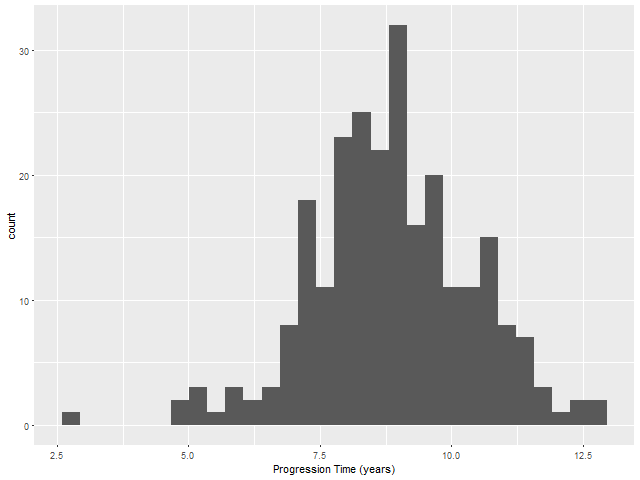
\includegraphics[width=0.8\textwidth]{sim_study_res_sc_10_sh_7pt5/progression_hist.png}
\caption{\label{fig : sc_10_sh_7pt5_progression_hist} Gleason reclassification times for patients from the test data set of scenario 1.}
\end{figure}

\begin{figure}[H]
\centering
\captionsetup{justification=centering}
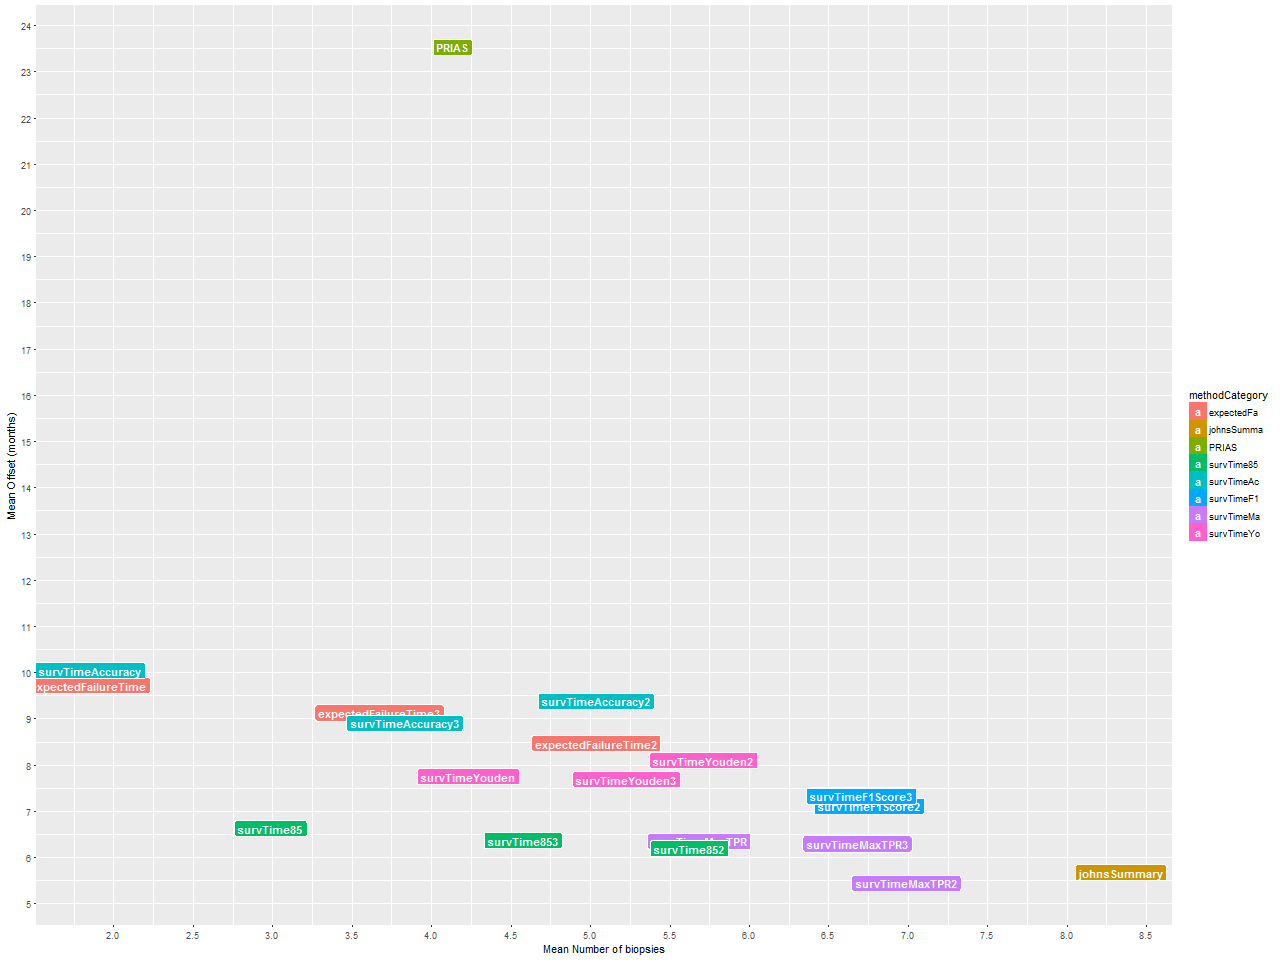
\includegraphics[width=\textwidth]{sim_study_res_sc_10_sh_7pt5/mean_offsetvsnb.png}
\caption{\label{fig : sc_10_sh_7pt5_mean_offsetvsnb} Mean number of biopsies against the mean offset (in years) for each of the approaches in scenario 1.}
\end{figure}

\begin{figure}[H]
\centering
\captionsetup{justification=centering}
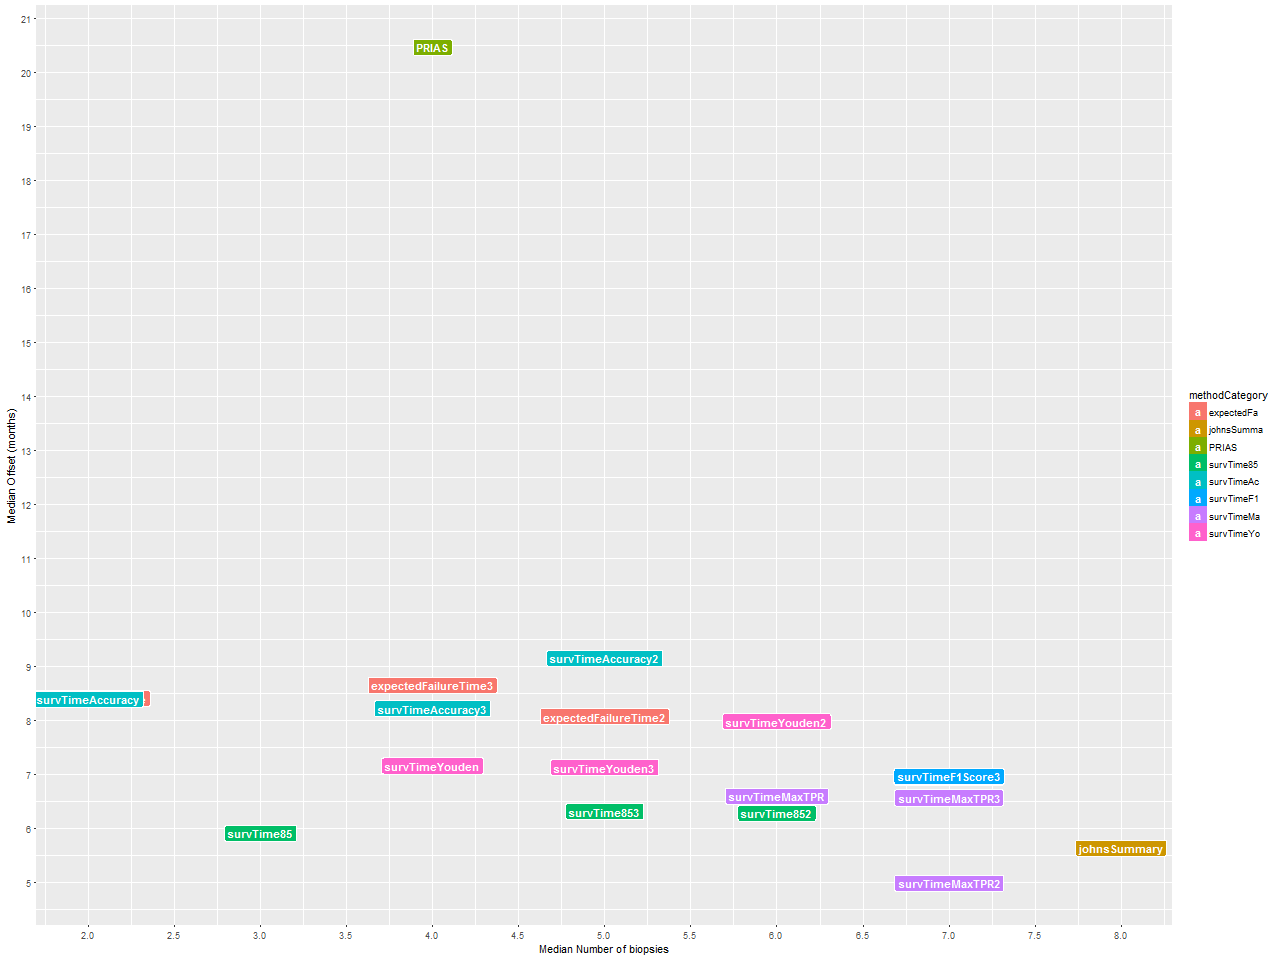
\includegraphics[width=\textwidth]{sim_study_res_sc_10_sh_7pt5/median_offsetvsnb.png}
\caption{\label{fig : sc_10_sh_7pt5_median_offsetvsnb}Median number of biopsies against the median offset (in years) for each of the approaches in scenario 1.}
\end{figure}

\begin{figure}[H]
\centering
\captionsetup{justification=centering}
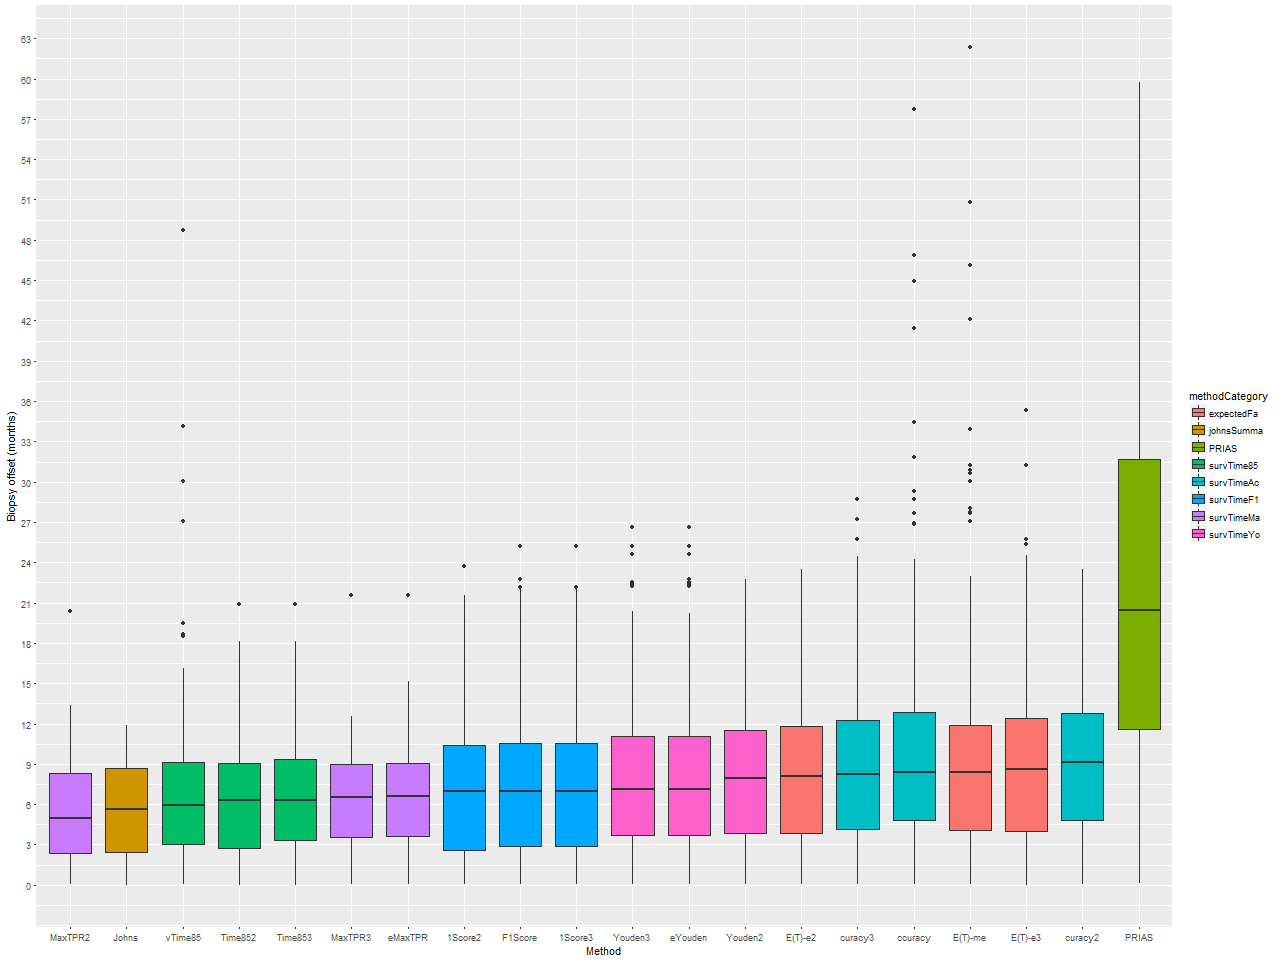
\includegraphics[width=\textwidth]{sim_study_res_sc_10_sh_7pt5/offset_boxplot.png}
\caption{\label{fig : sc_10_sh_7pt5_offset_boxplot} Boxplot for the offset corresponding to the various approaches in scenario 1.}
\end{figure}

\begin{figure}[H]
\centering
\captionsetup{justification=centering}
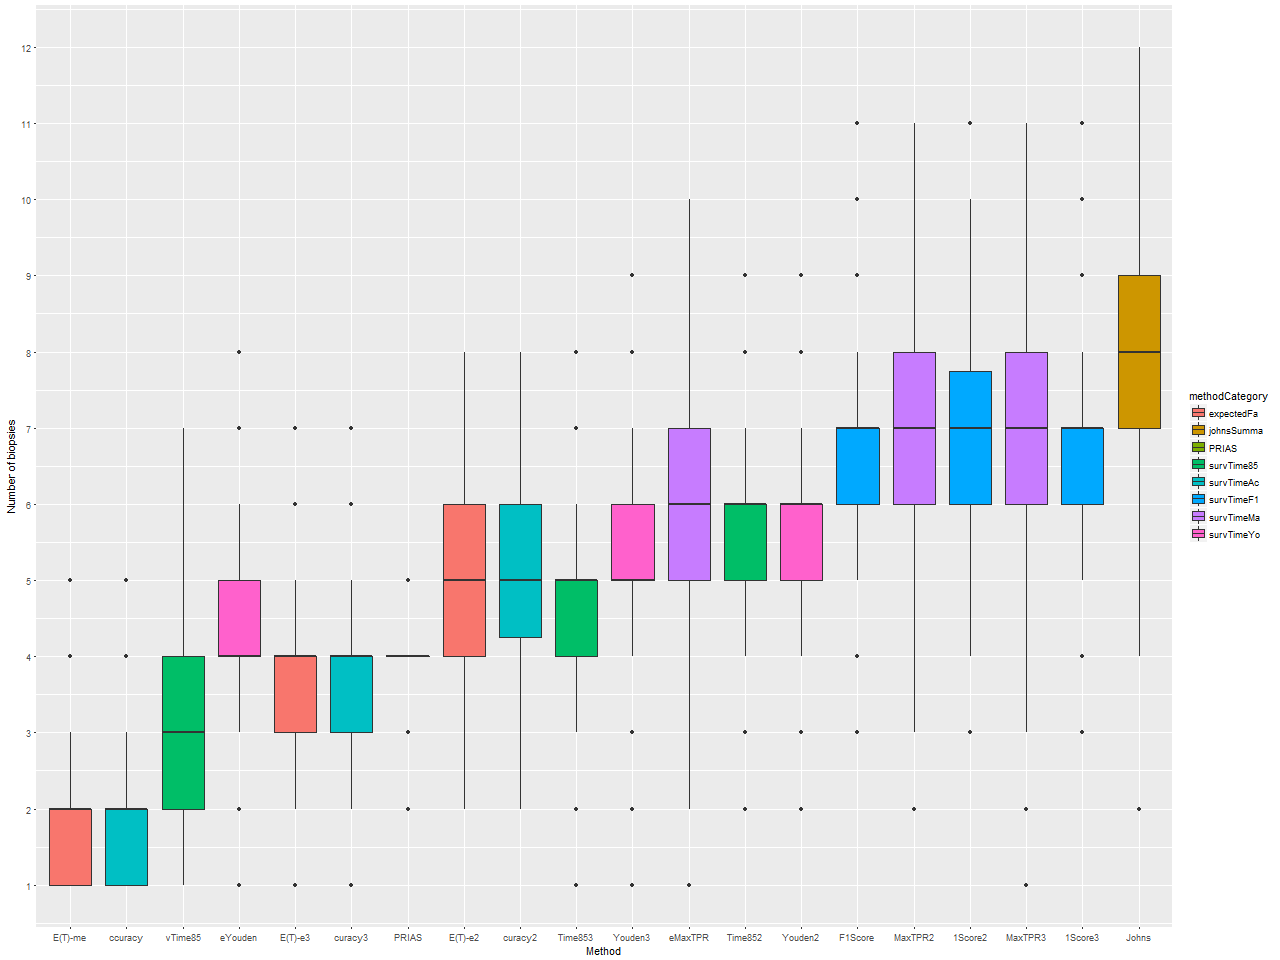
\includegraphics[width=\textwidth]{sim_study_res_sc_10_sh_7pt5/nb_boxplot.png}
\caption{\label{fig : sc_10_sh_7pt5_nb_boxplot} Boxplot for the number of biopsies corresponding to the various approaches in scenario 1.}
\end{figure}

\subsubsection{Scenario 2}
Unlike the previous scenario, the Gleason reclassification times for the patients in Scenario 2 are mostly between 0 and 5 years. The Gleason reclassification times of test patients from one of the data sets is shown in Figure \ref{fig : sc_6_sh_1pt5_progression_hist}. Figure \ref{fig : sc_6_sh_1pt5_offset_boxplot} shows that, for this data set the approach with the least number of biopsies is conditional expected failure time. The mean and median number of biopsies are 1.5 and 1 respectively. While the mean and median offset is around 18 months, there is considerable variation in the offset for the various patients. The first and third quartiles are at 12 months and 27 months respectively. The large variation in offset is due to the fact that time to Gleason reclassification has larger variance since it is based on a small history of the patient. In such a scenario one might be inclined towards doing a biopsy every year as they have the least offset. However that approach leads to a very large number of biopsies as shown in Figure \ref{fig : sc_6_sh_1pt5_nb_boxplot}. Certain approaches based on dynamic risk perform better here, both in terms of number of biopsies as well as the offset. In particular if the choice of $\kappa$ can be based on maximization of the Youden index or a fixed $\kappa$ can be chosen.

\begin{figure}[H]
\centering
\captionsetup{justification=centering}
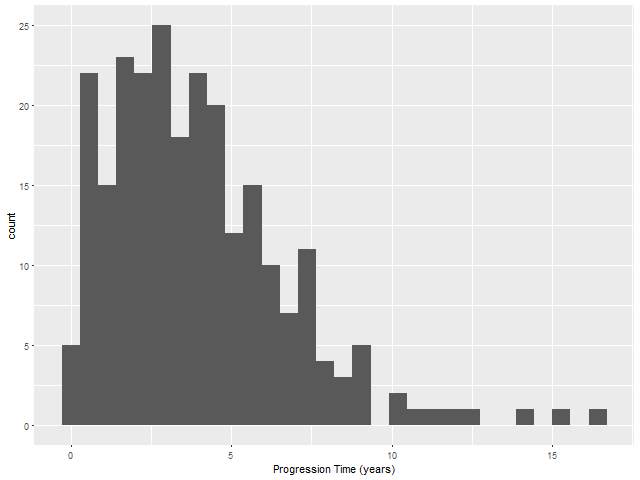
\includegraphics[width=0.8\textwidth]{sim_study_res_sc_6_sh_1pt5/progression_hist.png}
\caption{\label{fig : sc_6_sh_1pt5_progression_hist} Gleason reclassification times for patients from the test data set of scenario 2.}
\end{figure}

\begin{figure}[H]
\centering
\captionsetup{justification=centering}
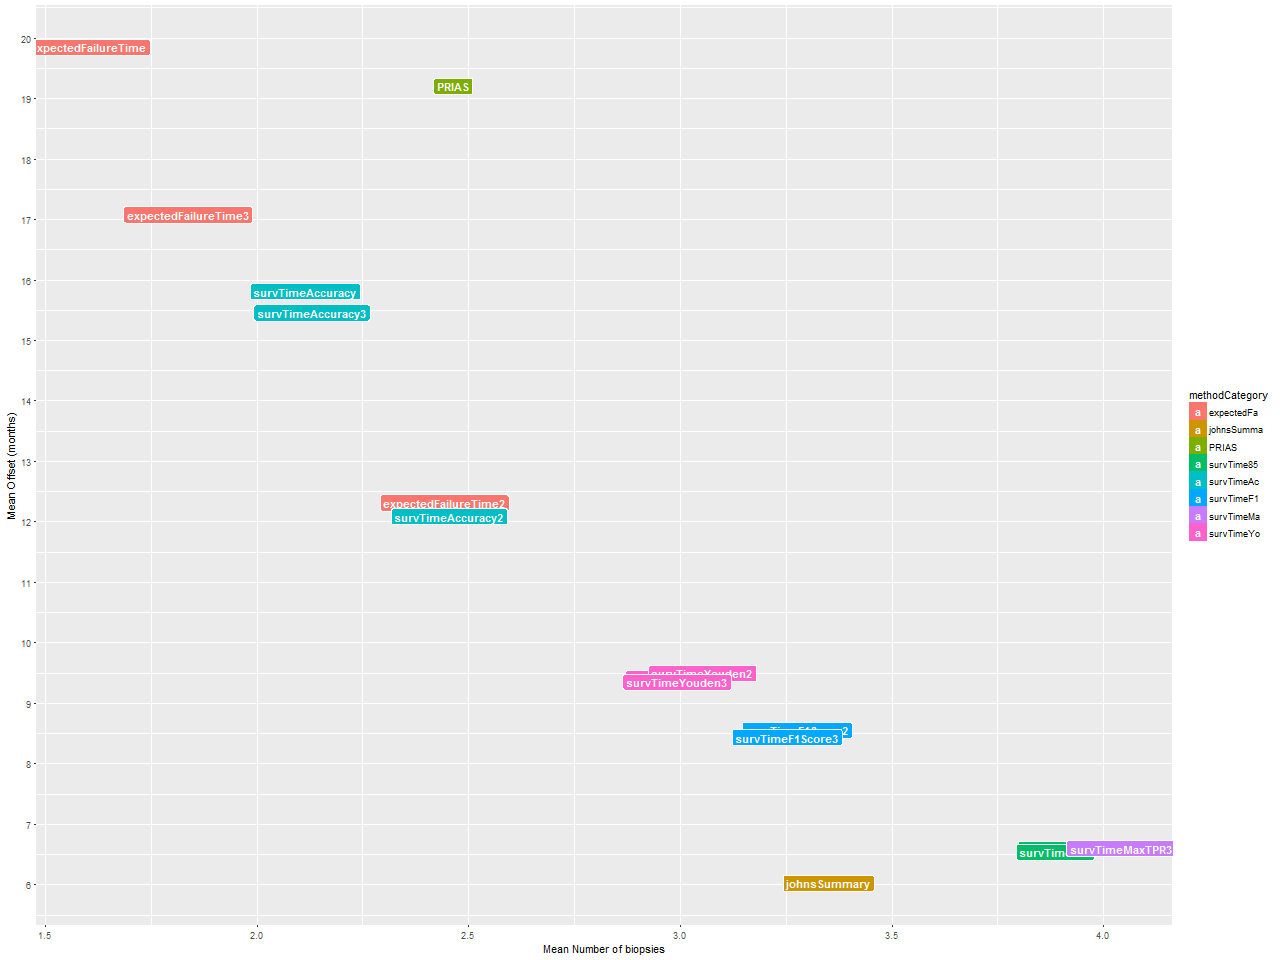
\includegraphics[width=\textwidth]{sim_study_res_sc_6_sh_1pt5/mean_offsetvsnb.png}
\caption{\label{fig : sc_6_sh_1pt5_mean_offsetvsnb} Mean number of biopsies against the mean offset (in years) for each of the approaches in scenario 2.}
\end{figure}

\begin{figure}[H]
\centering
\captionsetup{justification=centering}
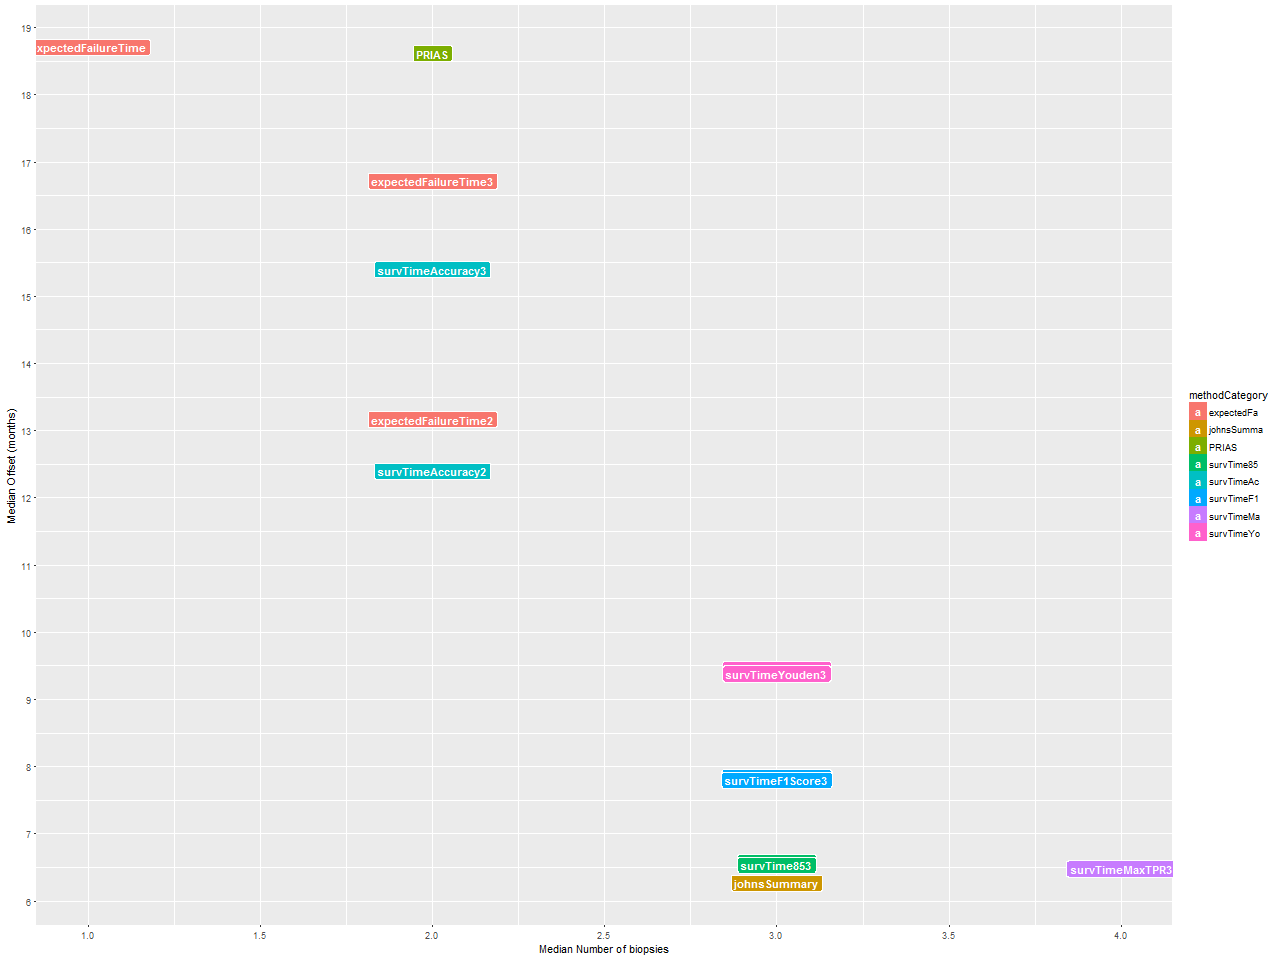
\includegraphics[width=\textwidth]{sim_study_res_sc_6_sh_1pt5/median_offsetvsnb.png}
\caption{\label{fig : sc_6_sh_1pt5_median_offsetvsnb}Median number of biopsies against the median offset (in years) for each of the approaches in scenario 2.}
\end{figure}

\begin{figure}[H]
\centering
\captionsetup{justification=centering}
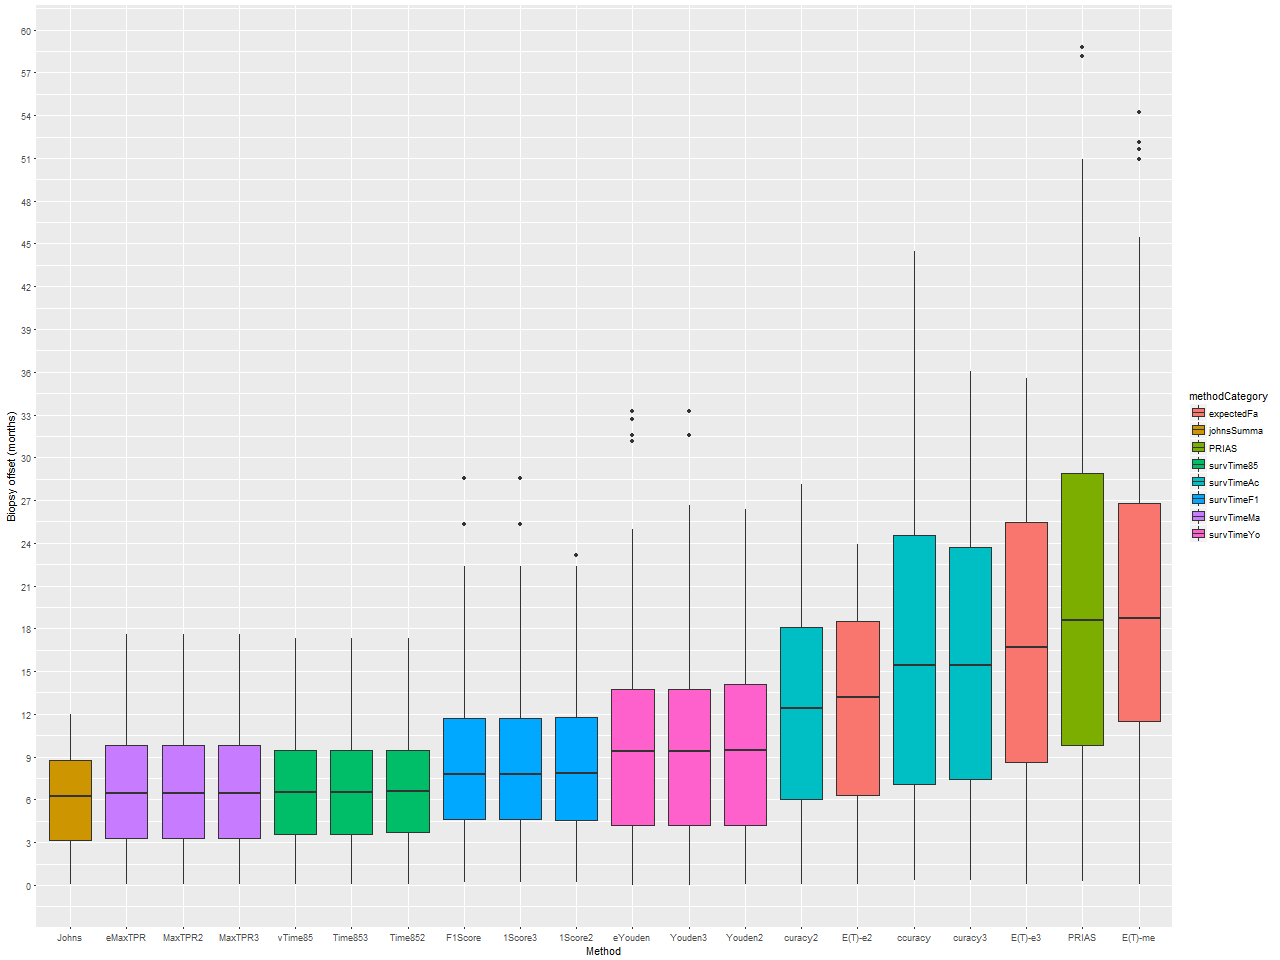
\includegraphics[width=\textwidth]{sim_study_res_sc_6_sh_1pt5/offset_boxplot.png}
\caption{\label{fig : sc_6_sh_1pt5_offset_boxplot} Boxplot for the offset corresponding to the various approaches in scenario 2.}
\end{figure}

\begin{figure}[H]
\centering
\captionsetup{justification=centering}
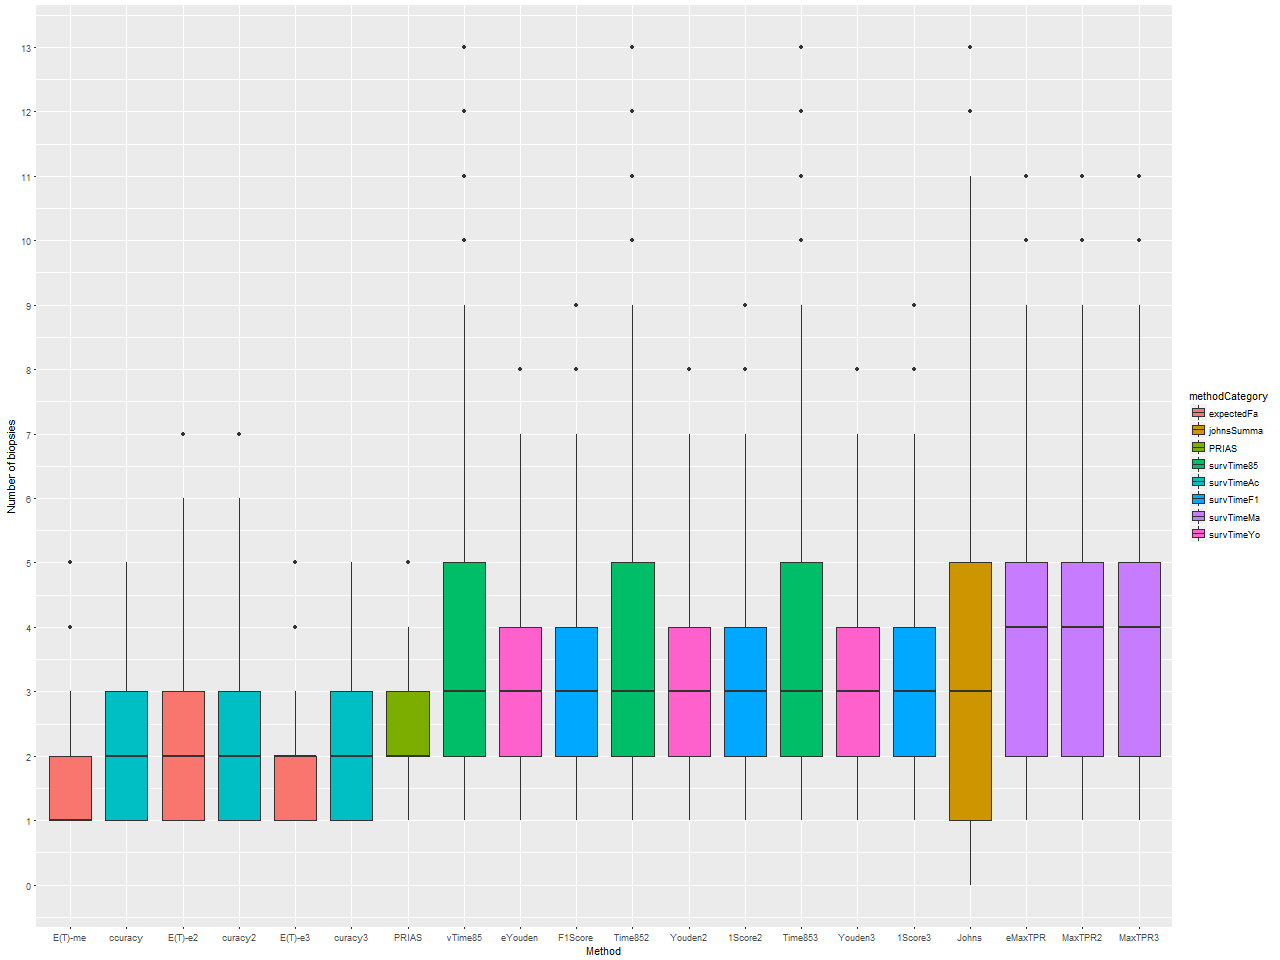
\includegraphics[width=\textwidth]{sim_study_res_sc_6_sh_1pt5/nb_boxplot.png}
\caption{\label{fig : sc_6_sh_1pt5_nb_boxplot} Boxplot for the number of biopsies corresponding to the various approaches in scenario 2.}
\end{figure}

\subsubsection{Scenario 3}
In scenario 3, the Gleason reclassification times for the patients are widely spread, mostly between 2 and 9 years. i.e. patients fail late as well early. The Gleason reclassification times of test patients from one of the data sets is shown in Figure \ref{fig : sc_8pt5_sh_3_progression_hist}. Figure \ref{fig : sc_8pt5_sh_3_offset_boxplot} shows that, for this data set the approach with the least number of biopsies is conditional expected failure time. The mean and median number of biopsies are 1.5 and 1 respectively. This method also has considerable variation in the offset for the various patients. The first and third quartiles are at 9 months and 27 months respectively. A more detailed analysis revealed that the variation in offset was higher for subjects with earlier failure times. For e.g. the mean and median offset in subjects with reclassification times more than 4 years was nearly 13.5 months. For others it was nearly 39.5 months. This is once again is due to the fact that time to Gleason reclassification has larger variance since it is based on a small history of the patient. And thus usefulness of conditional expected failure time is questionable.\\

Dynamic risk based methods once again provide an alternative. If a fixed $\kappa$ of 0.15 is used then although the offset will be low, there is very high variation in number of biopsies. i.e. people who have reclassifications early will benefit but people who have reclassifications later will have too many biopsies. If $\kappa$ is chosen such that accuracy is maximized, and a biopsy is done whenever there is a gap of 2 years then a reasonable offset is obtained. The first and third quartiles are almost 4.5 and 18 months. The first and third quartiles for number of biopsies are 3 and 4. 

\begin{figure}[H]
\centering
\captionsetup{justification=centering}
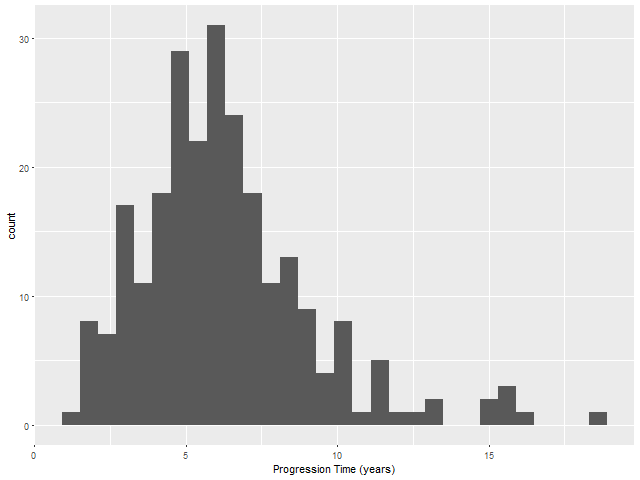
\includegraphics[width=0.8\textwidth]{sim_study_res_sc_8pt5_sh_3/progression_hist.png}
\caption{\label{fig : sc_8pt5_sh_3_progression_hist} Gleason reclassification times for patients from the test data set of scenario 3.}
\end{figure}

\begin{figure}[H]
\centering
\captionsetup{justification=centering}
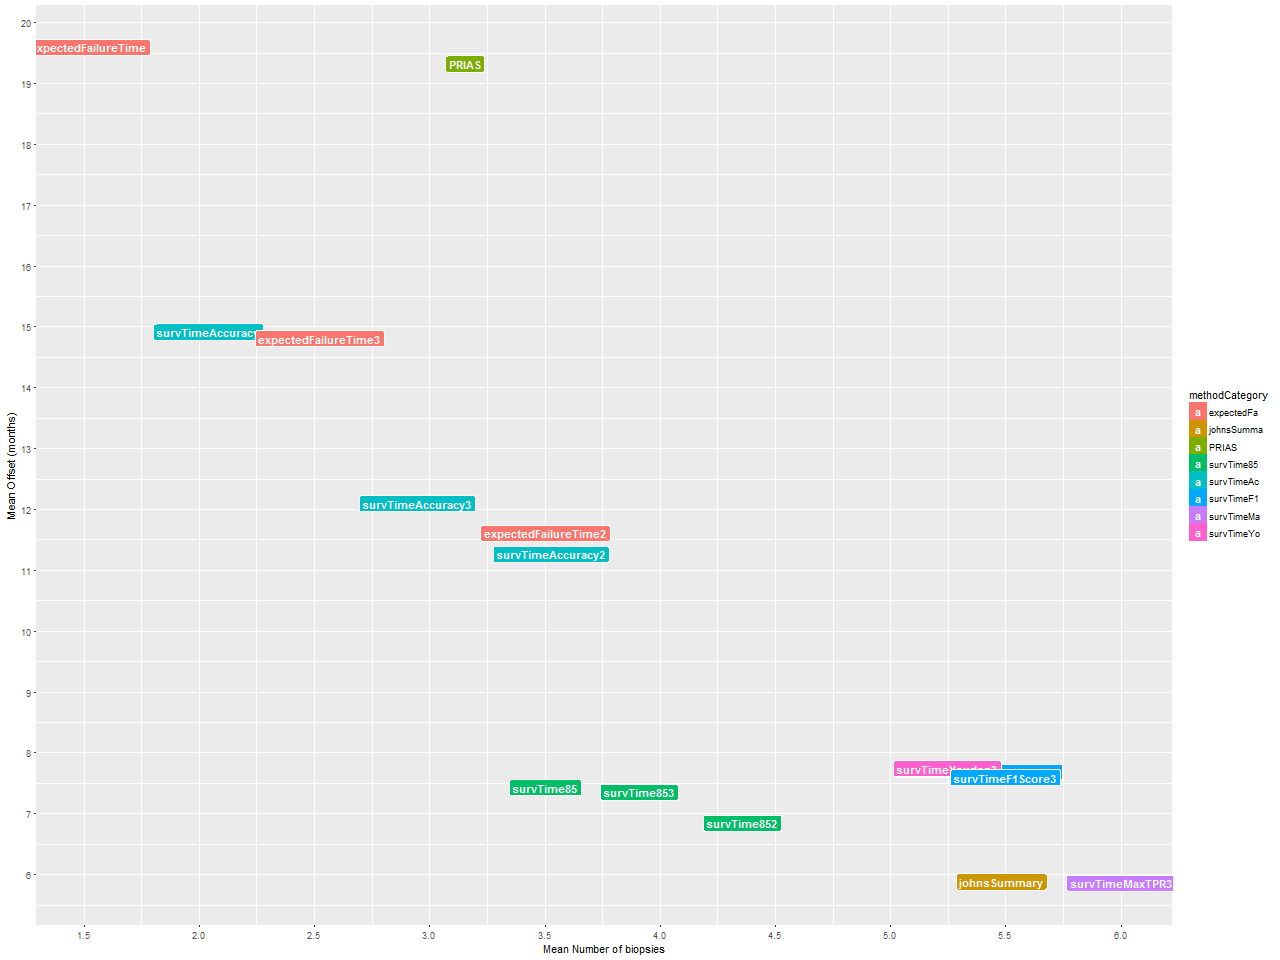
\includegraphics[width=\textwidth]{sim_study_res_sc_8pt5_sh_3/mean_offsetvsnb.png}
\caption{\label{fig : sc_8pt5_sh_3_mean_offsetvsnb} Mean number of biopsies against the mean offset (in years) for each of the approaches in scenario 3.}
\end{figure}

\begin{figure}[H]
\centering
\captionsetup{justification=centering}
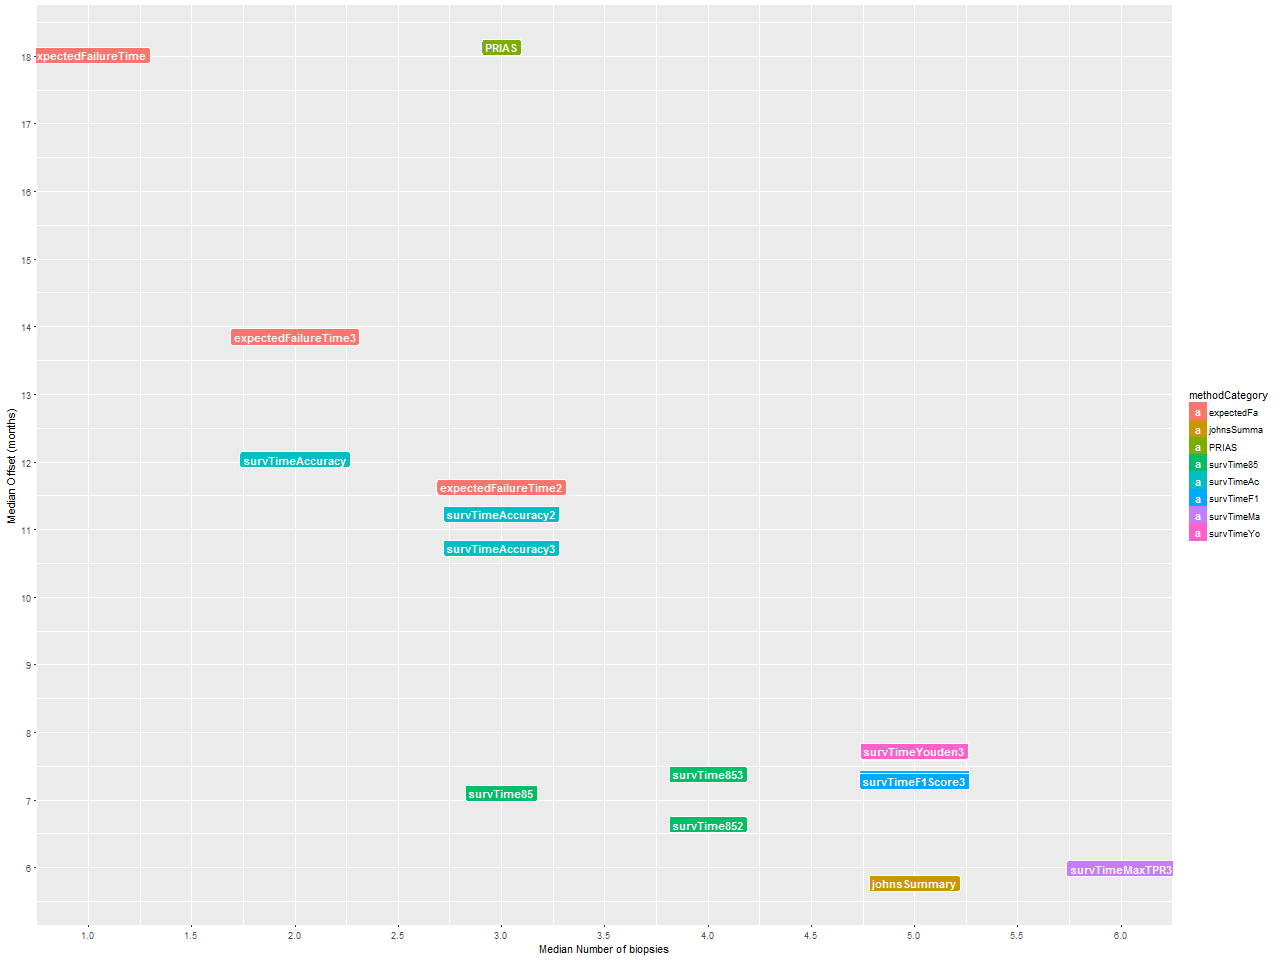
\includegraphics[width=\textwidth]{sim_study_res_sc_8pt5_sh_3/median_offsetvsnb.png}
\caption{\label{fig : sc_8pt5_sh_3_median_offsetvsnb}Median number of biopsies against the median offset (in years) for each of the approaches in scenario 3.}
\end{figure}

\begin{figure}[H]
\centering
\captionsetup{justification=centering}
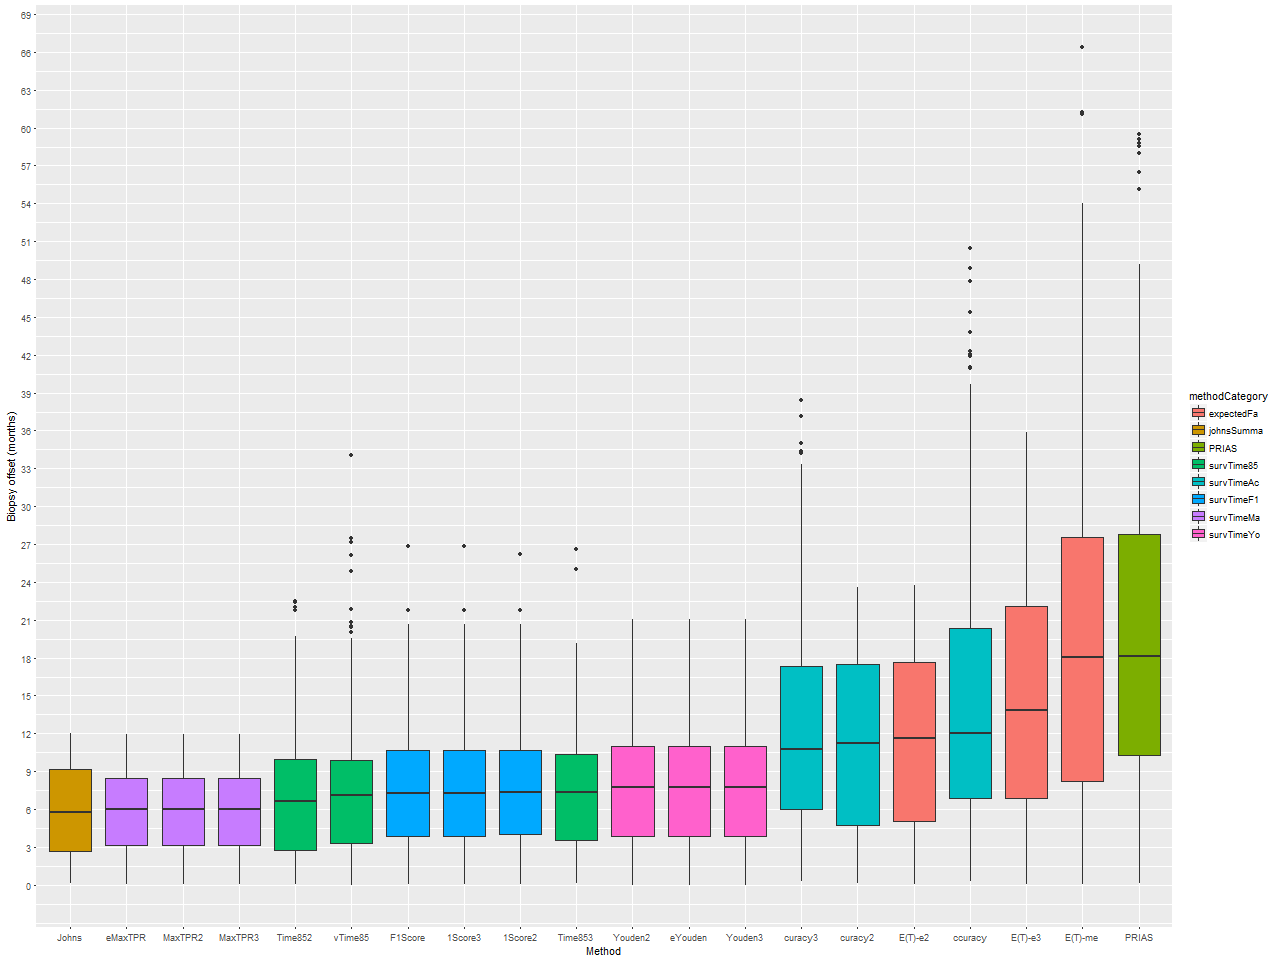
\includegraphics[width=\textwidth]{sim_study_res_sc_8pt5_sh_3/offset_boxplot.png}
\caption{\label{fig : sc_8pt5_sh_3_offset_boxplot} Boxplot for the offset corresponding to the various approaches in scenario 3.}
\end{figure}

\begin{figure}[H]
\centering
\captionsetup{justification=centering}
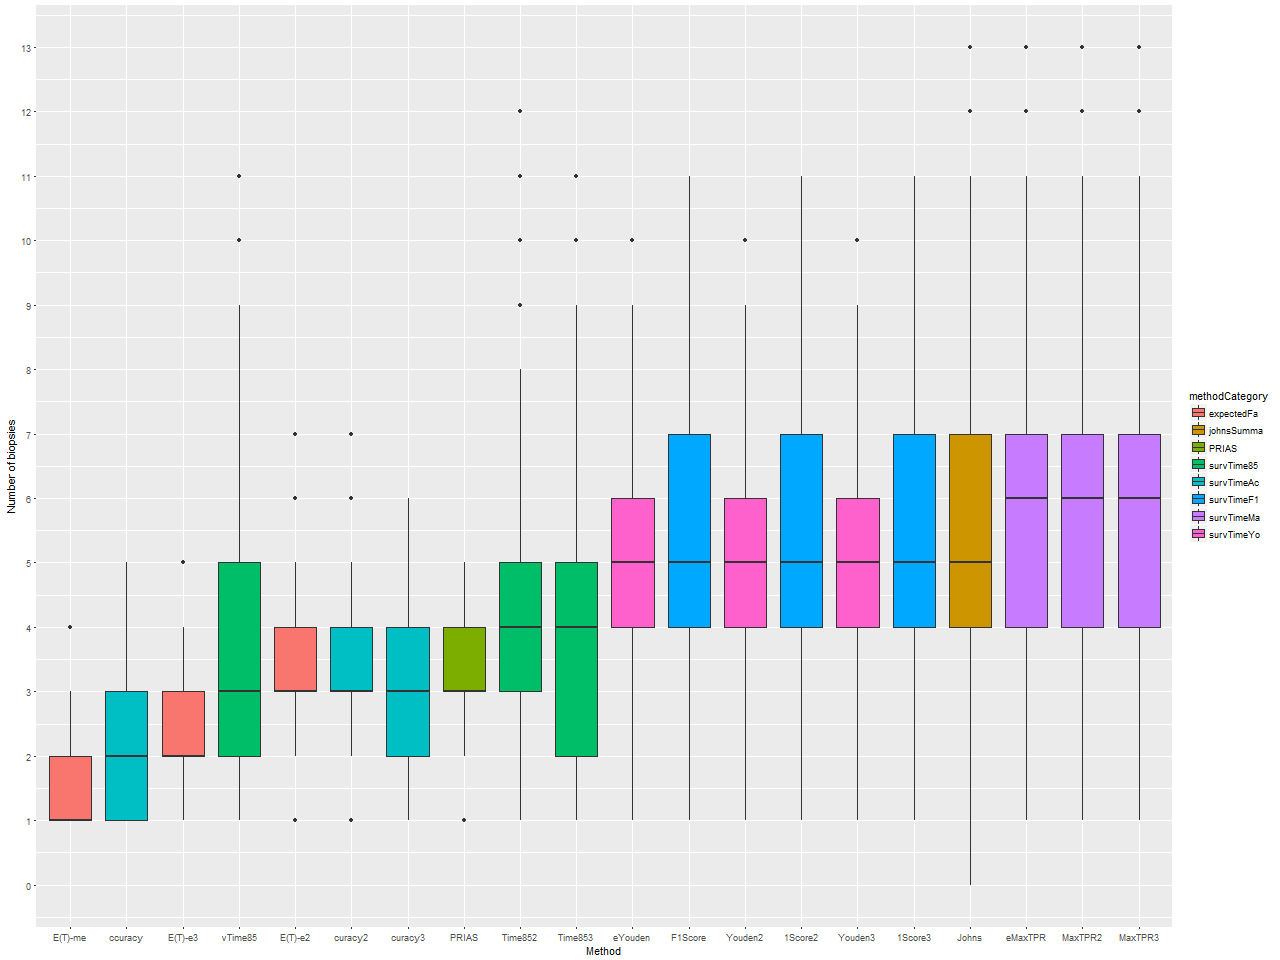
\includegraphics[width=\textwidth]{sim_study_res_sc_8pt5_sh_3/nb_boxplot.png}
\caption{\label{fig : sc_8pt5_sh_3_nb_boxplot} Boxplot for the number of biopsies corresponding to the various approaches in scenario 3.}
\end{figure}

\subsection{A mixed approach: E(T) vs dynamic risk}
While we did create biopsy schedules using conditional expected Gleason reclassification time, and dynamic risk of Gleason reclassification based approaches, we saw that no single approach works best in all scenarios. In particular, we observed that when the failure times are early dynamic risk based approaches perform better in terms of offset than conditional expected Gleason reclassification time. The latter works best when the Gleason reclassification times are later. This has motivated us to use a mixed approach, where we schedule biopsies using dynamic risk based approaches if the variance (Eq. \ref{eq : varFailureTime}) of time to Gleason reclassification is higher than a certain threshold, otherwise we use conditional expected Gleason reclassification time. This is still work in progress.